\documentclass{beamer}
\usepackage[latin1]{inputenc}
\usetheme{Goettingen}
\title[LP Relaxations]{Linear Programming Relaxations \\ Or, how I learned to stop worrying and love SDP}
\author{Nic Hollingum}
\institute{USYD}
\begin{document}

\begin{frame}
\titlepage
\end{frame}

\begin{frame}{Outline}
\begin{itemize}
	\item Problems
	\item IP/LP Formulations
	\item Linearity Gap
	\item Maxflow Obstacles
	\item RAAP Obstacles
\end{itemize}
\end{frame}

%-----------------------------------------------------------------------------------
\section{The Problems}

\begin{frame}{Max-Cut}
\begin{columns}
\begin{column}{6cm}
\begin{itemize}
	\item Given a graph $G=(V,E)$
	\item partition the vertices into 2 sets $A, B$.
	\item such that the number of edges with endpoints in both sets is maximised.
\end{itemize}
\end{column}
\begin{column}{4cm}
\center{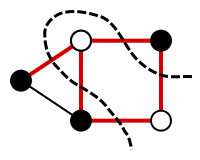
\includegraphics[width=4cm]{../res/maxcut.png}}
\end{column}
\end{columns}
\end{frame}

\begin{frame}{Robust Actor Allocation}
\begin{columns}
\begin{column}{6cm}
\begin{itemize}
	\item Given a computational graph $G=(V,E)$ and a set of processors $P$.
	\item Map the vertices to the processors
	\item such that:
	\begin{itemize}
		\item The total time spend processing and communicating is minimised
		\item No actors which are duplicates of each other reside on the same processor
	\end{itemize}
\end{itemize}
\end{column}
\begin{column}{4cm}
\center{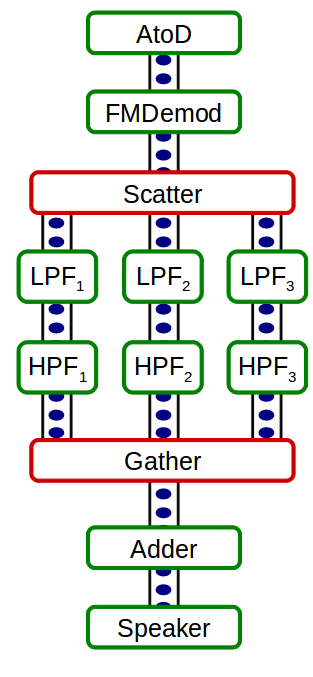
\includegraphics[width=4cm]{../res/multiradio.png}}
\end{column}
\end{columns}
\end{frame}

%-----------------------------------------------------------------------------------
\section{The Integer Programmes}

\begin{frame}{Max-Cut I}
\begin{align}
	\nonumber Maximize: & \sum_{(i,j) \in E}{x_i + x_j - 2 x_i x_j} \\
	\nonumber s.t. & \\
	\nonumber & x \in \{0,1\}^{|V|}
\end{align}
\end{frame}

\begin{frame}{Robust Actor Allocation I}
\begin{align}
	\nonumber Minimize: & \sum_{(a,b) \in E; p,q \in P} \mathbf{C}_{a,b,p,q}\mathbf{X}_{a,p}\mathbf{X}_{b,q} \\
	\nonumber & + \sum_{a \in V; p \in P} \mathbf{I}_{a,p}\mathbf{X}_{a,p} \\
	\nonumber s.t. &  \\
	\nonumber & \forall a \in V : \sum_{p \in P}\mathbf{X}_{a,p} = 1 \\
	\nonumber & \forall a,b \in V : \sum_{p \in P}\mathbf{X}_{a,p}\mathbf{X}_{b,p}\mathbf{D}_{a,b} = 0
\end{align}
\end{frame}

\begin{frame}{Quadratic Terms}
\begin{columns}
\begin{column}{5cm}
\begin{itemize}
	\item These LP's cant be solved by a lienar programme solver
	\item $X_i X_j$ is a quadratic term
	\begin{itemize}
		\item curved solution space
		\item solver can't deal with points along the curved hyper-surface
	\end{itemize}
	\item Must Linearise
\end{itemize}
\end{column}
\begin{column}{5cm}
\center{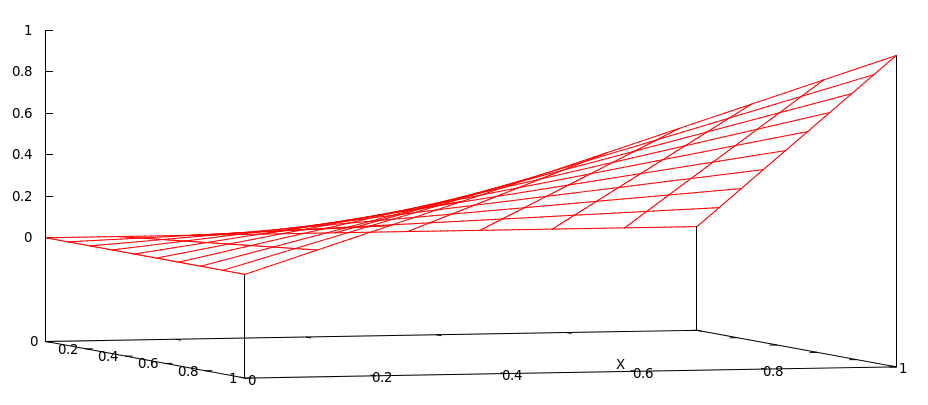
\includegraphics[width=5cm]{../res/quadratic.png}}
\end{column}
\end{columns}
\end{frame}

\begin{frame}{Quadratic Terms}
\begin{columns}
\begin{column}{5cm}
\center{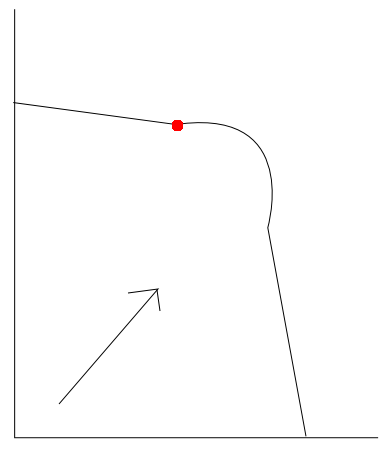
\includegraphics[width=5cm]{../res/quad1.png}}
\end{column}
\begin{column}{5cm}
\center{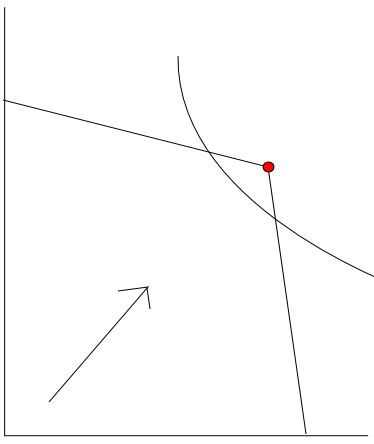
\includegraphics[width=5cm]{../res/quad2.png}}
\end{column}
\end{columns}
\end{frame}

\begin{frame}{Max-Cut II}
\begin{align}
	\nonumber Maximize: & \sum_{i,j \in V}{y_{i,j}e_{i,j}} \\
	\nonumber s.t. & \\
	\nonumber & y_{i,j} <= y_{i,k} + y_{k,j} \\
	\nonumber & y_{i,j} + y_{i,k} + y_{k,j} <= 2 \\
	\nonumber & y \in \{0,1\}^{|V|, |V|}
\end{align}
\end{frame}

\begin{frame}{Robust Actor Allocation II}
\begin{align}
	\nonumber Minimize: & \sum_{a,b \in V; p,q \in P} \mathbf{C}_{a,b,p,q}\mathbf{Y}_{a,b,p,q} \\
	\nonumber & + \sum_{a \in V; p \in P} \mathbf{I}_{a,p}\mathbf{X}_{a,p} \\
	\nonumber s.t. &  \\
	\nonumber & \forall a \in V : \sum_{p \in P}X_{a,p} = 1 \\
	\nonumber & \forall a,b \in V : \forall p,q \in P : \quad \mathbf{Y}_{a,b,p,q} \leq \mathbf{X}_{a,p} \\
	\nonumber & \forall a,b \in V : \forall p,q \in P : \quad \mathbf{Y}_{a,b,p,q} \leq \mathbf{X}_{b,q} \\
	\nonumber & \forall a,b \in V : \forall p,q \in P : \quad \mathbf{X}_{a,p} + \mathbf{X}_{b,q} - 1 \leq \mathbf{Y}_{a,b,p,q} \\
	\nonumber & \forall a,b \in V : \sum_{p \in P}\mathbf{Y}_{a,b,p,p}\mathbf{D}_{a,b} = 0
\end{align}
\end{frame}

%-----------------------------------------------------------------------------------
\section{Linearity Gap}

\begin{frame}{Solution Polytopes}
\begin{columns}
\begin{column}{6cm}
\begin{itemize}
	\item Feasible solution region
	\item LP solver tries to find extreme points
	\begin{itemize}
		\item Simplex
		\item Interior point
	\end{itemize}
	\item Linear polytope is larger
\end{itemize}
\end{column}
\begin{column}{4cm}
\center{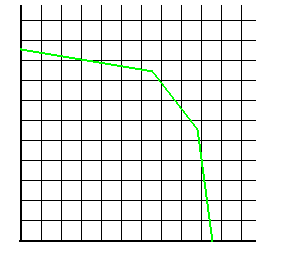
\includegraphics[width=4cm]{../res/linear.png}}
\end{column}
\end{columns}
\end{frame}

\begin{frame}{Linearity Gap}
\begin{columns}
\begin{column}{6cm}
\begin{itemize}
	\item Arises when decision variable is allowed to take a real value
	\item Margin between Integral polytope and its linear relaxation
	\item Known size for some problems
\end{itemize}
\end{column}
\begin{column}{4cm}
\center{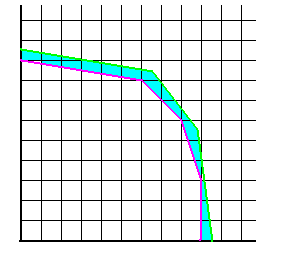
\includegraphics[width=4cm]{../res/gap.png}}
\end{column}
\end{columns}
\end{frame}

\begin{frame}{Approximating the gap}
\begin{columns}
\begin{column}{6cm}
\begin{itemize}
	\item Plane cutting
	\item Restrict linear polytope closer to integral one
	\item Informal method, difficult to reason about time
\end{itemize}
\end{column}
\begin{column}{4cm}
\center{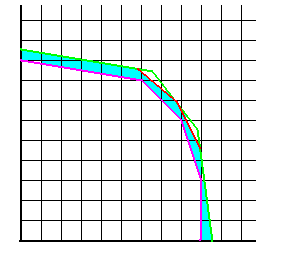
\includegraphics[width=4cm]{../res/closing.png}}
\end{column}
\end{columns}
\end{frame}

\begin{frame}{Sherali-Adams}
\begin{itemize}
	\item {\em Lift and Project}
	\item Systematic method of closing the gap
	\item Guaranteed to converge after n steps
	\item Requires time polynomial in the number of steps to run
	\item allows us to reason more strongly about integrality gap
\end{itemize}
\end{frame}

%-----------------------------------------------------------------------------------
\section{Failures in Maxcut Land}

\begin{frame}{Polytope Difference}
\begin{itemize}
	\item Maxcut's integrality gap is $2-\epsilon$
	\item Difference is not intuitively ingrained
	\item Unique Games Conjecture: 1/.878
\end{itemize}
\end{frame}

\begin{frame}{Old Information}
\begin{columns}
\begin{column}{6cm}
\begin{itemize}
	\item Lift and Project adds dimensions to restrict solution
	\item Variables in new dimensions must have slack
	\item Lifted variables are automatically tight
	\item New constraints arent contained in the polytope
\end{itemize}
\end{column}
\begin{column}{4cm}
\center{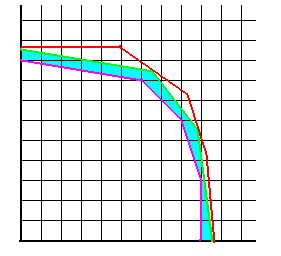
\includegraphics[width=4cm]{../res/nonew.png}}
\end{column}
\end{columns}
\end{frame}

\begin{frame}{Negative Result}
\begin{itemize}
	\item Result shows that Sherali-Adams L \& P doesn't work for MAXCUT \cite{fer07}
	\begin{itemize}
		\item Fixed steps: doesn't lower bound
		\item Variable steps: lowers bound, exponential time
	\end{itemize}
	\item Special case: dense graphs ($1 + \epsilon$)
	\item APX-Hard
\end{itemize}
\end{frame}

%-----------------------------------------------------------------------------------
\section{Failures in RAAP Land}

\begin{frame}{Infinite gap}
\begin{columns}
\begin{column}{6cm}
\begin{itemize}
	\item Linear relaxation has a big gap
	\item Quadratic term
	\begin{itemize}
		\item $0.5 \times 0.5 = 0.25$
		\item $min[0, 0.5] = 0$
	\end{itemize}
	\item LP solver defeats itself
	\item weak model
\end{itemize}
\end{column}
\begin{column}{4cm}
\center{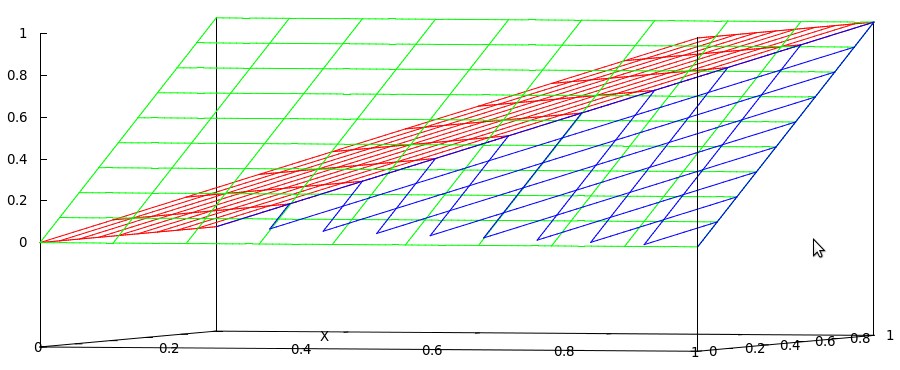
\includegraphics[width=4cm]{../res/approx.png}}
\end{column}
\end{columns}
\end{frame}

\begin{frame}{Trivial bound}
\begin{columns}
\begin{column}{6cm}
\begin{itemize}
	\item Gap of infinite size
	\item Trivial solution infinitely different from optimal
	\item solvable in constant time
	\item Requires a stronger model
	\item We don't suspect RAAP is APX-Hard
\end{itemize}
\end{column}
\begin{column}{4cm}
\center{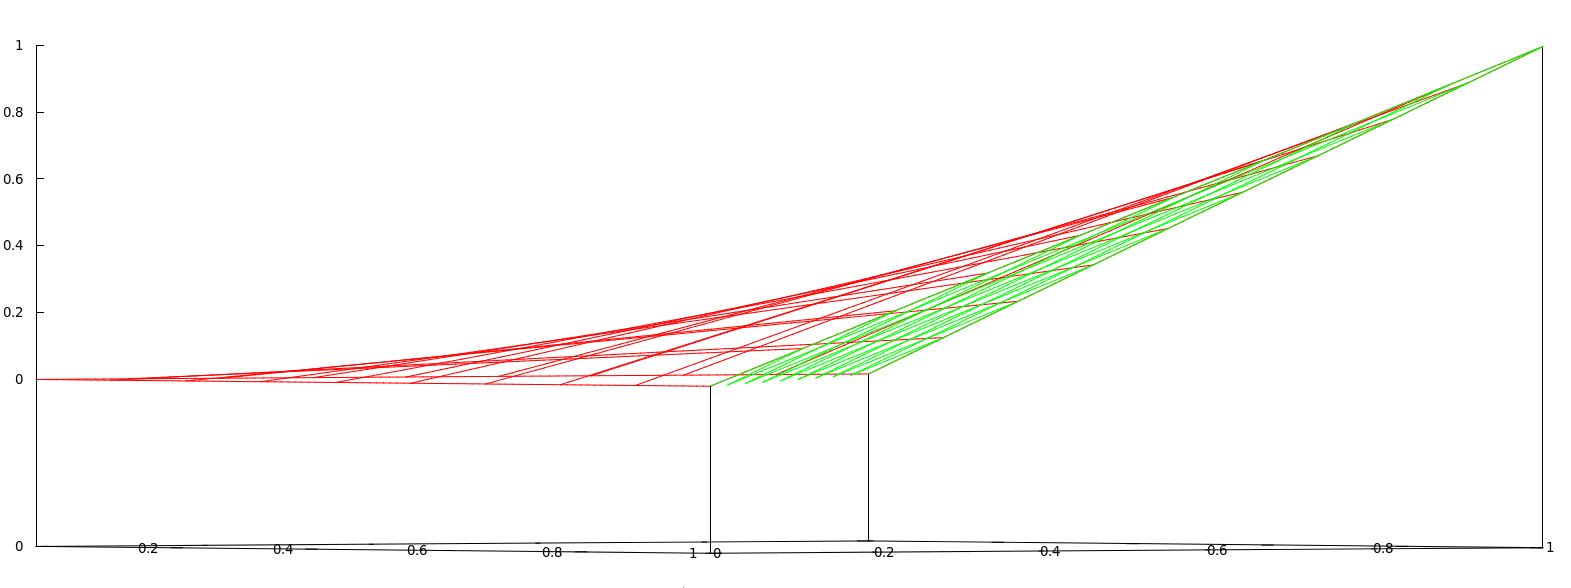
\includegraphics[width=4cm]{../res/infinitegap.png}}
\end{column}
\end{columns}
\end{frame}

%-----------------------------------------------------------------------------------
\section{Conclusions}

\begin{frame}{In Conclusion}
\begin{itemize}
	\item Integrality gap is a major issue
	\item Not always closable
	\item Sometimes will break the relaxation
	\item Use Semidefinite Programming
\end{itemize}
\end{frame}

\begin{frame}[allowframebreaks]{References}
\bibliographystyle{wmaainf}
\bibliography{biblio}
\end{frame}

\begin{frame}{Questions?}
\end{frame}

\end{document}
